%% ----------------------------------------------------------------
%% Theory.tex
%% 5398
%% ---------------------------------------------------------------- 
\chapter{Background theory \& literature review} \label{Chapter: Theory}

%Check that you provide enough background information: your reader does not know what you know. Assuming that your reader knows much more than you and therefore omitting background information is a widespread problem with students.

%Many students seem to think that they know little while everyone else knows a lot —therefore they shouldn’t explain things that everyone probably already knows. It is only later in their careers when they realise that no-one really knows that much! Besides, there will be readers from adjacent (sub)fields and readers who are just learning the tricks of the trade. Use a colleague who works on something slightly different than you as a test reader —ask her which parts of the text are hard to follow, and revise accordingly.

%\begin{enumerate}
%\item Setting the scene
%\item Underlying information
%\end{enumerate}

\section{Deep Learning}

The Deep Learning term was created in contrast to ``shallow" Machine Learning. Typical machine learning algorithms involve processing the information from the input into a different \textit{feature space} in which the data is represented in a more structured way. With deep learning, this process is repeated several times allowing for feature spaces with higher-level abstractions that have more power to learn complex relations in the input (\cite{Goodfellow-et-al-2016}). In the beginning, neural networks would only have a single hidden layer of neurons. Theoretically, one layer should suffice for learning any continuous function, according to the \textit{universal approximation theorem} (\cite{Cybenko1989}), provided that the network has enough hidden units. However, the number of necessary units for reaching a certain accuracy can grow exponentially with the input space (\cite{Barron1993}), which can only be alleviated by increasing the depth of the system. Bigger networks were hard to train at the beginning because of an increased number of parameters that significantly extend the computation training time, a higher risk to over-fit due to their increased power, \textit{vanishing gradients} ---meaning that lower-layer parameters receive weak signals from the error and could barely learn--- and their need for vast amounts of data, not readily available at the time. Such problems have been recently overcome thanks to the use of Graphical Processing Units (GPUs) that boost computing speed, techniques such as \textit{dropout} (\cite{Srivastava2014}) and \textit{batch normalization} (\cite{SergeyIoffe2015}) that add extra regularization, the inclusion of Rectifying Linear Units (ReLUs) as non-linear functions, and the increased amount of data available thanks to the Big Data broader movement. Since then, its use has been growing, and it has spread to many research fields, with high performance in image classification ---improvement of 10\% from previous methods (\cite{NIPS2012_4824})---, speech recognition ---more than 5\% improvement (\cite{Vesely2013})--- and language translation --more than 1 point BLEU score increase (\cite{Cho2014})---.

Multi-Layer Perceptrons (MLPs), Recurrent Neural Networks (RNNs) and Convolutional Neural Networks (CNNs) can be found among the most widespread deep networks. MLPs are composed of consecutive layers of fully-connected units that pass the information in one direction and hence are called \textit{feedforward}. RNNs differ from MLPs in that units are also allowed to have connections to themselves. Instead of having an input vector that produces an output in a \textit{one-go} fashion, RNNs store information from previous inputs and are particularly well-suited for inputs that are sequentially correlated. CNNs slide a local filter throughout the input, allowing obtaining location-invariant information. A more in-depth look into this kind of network is shown in the following sub-section.

\subsection{Convolutional Neural Networks} \label{sect:cnn}
As mentioned above, CNNs (\cite{LeCun1998}) work by having filters that operate along some spatially correlated input. Filters are small patches that hold one weight per position. They perform element-wise multiplication with a patch from the input of the same size and add them up into a single output that is located at its centre. A non-linear function is then applied to the output space in order to obtain more expressive models. By performing this operation at all possible overlapping input patches, they produce a feature map that is somehow linked to the underlying input space. Since the same small filter is applied to the whole input space, they capture features or motifs that are location-independent. Moreover, just a small set of weights is used for an arbitrarily large input space, making them much more efficient and able to build deeper networks.

When defining a convolution operation, two extra parameters need to be taken into account: \textit{padding} and \textit{strides}. Padding consists of augmenting the input space by adding margins with zero value. It is especially useful for preserving the size of the input into the feature space, which is done by adding a margin of half of the filter size. The strides define the size of the steps taken every time the filter is slid, determining the amount of overlapping in the produced feature map. Figure \ref{fig:padding} shows a simple schematic of how a filter with padding and strides works.

\begin{figure}
	\centering
	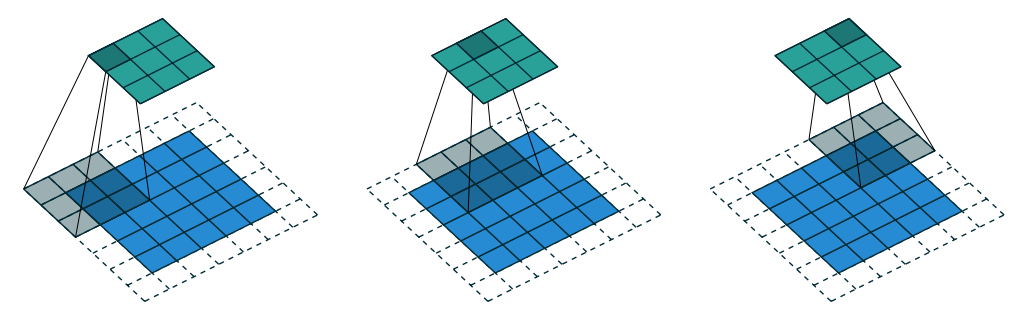
\includegraphics[width=0.8\linewidth]{Figures/padding}
	\caption{\textit{Convolution operation with a 3x3 filter, padding of 1x1 and strides of 2x2}. The blue cells represent the input space, the white ones are the result of padding, and the green cells form the output space. The filter operation is performed on the shaded input cells and produces the shaded output cells. Due to the strides, the filter jumps two positions while sliding. Figure reproduced from \cite{Dumoulin2016}.}
	\label{fig:padding}
\end{figure}

A convolutional layer typically includes a few sets of filters with varying size, producing a set of feature maps. Convolutional layers stack onto each other, building more and more abstract concepts. They can also be interleaved by pooling layers that shrink the maps by applying operations to their inputs in a similar fashion as the filters. Typical pooling operations are \textit{max-pool}, which takes the maximum value in a patch, or \textit{average pooling}, which averages overall units in the patch. The whole structure can be capped by a fully-connected MLP that performs a classification task, and all the weights trained by \textit{backpropagation}.

CNNs have found increased use in the last few years, thanks to advances in the techniques to build them that led to more sophisticated networks. They have had particular success for the tasks of image classification, object detection, text recognition, speech recognition, natural language processing, among others (\cite{Gu2017}).

\subsection{Drawbacks of deep-learning}
Despite the benefits of improved performance, deep learning still finds some resistance in the broader public due to varied reasons. First, its higher complexity imposes a steeper learning curve. Second, the lack of a mature set of tools and samples due to its novelty makes its access difficult, although there has been an increasing, active community that is swiftly covering these needs. Third, the high computational times are only partially relieved by GPUs. Last, deep networks are hard to interpret and obtaining information from the middle layers renders futile. Their \textit{black box} behaviour hinders developers understanding both where networks fail and why specific outputs are produced. This drawback has been of big concern lately, and the research community has switched the focus to developing \textit{interpretability techniques} to overcome it.

%"Deep neural networks are highly expressive models that have recently achieved state of the art performance on speech and visual recognition tasks. While their expressiveness is the reason they succeed, it also causes them to learn uninterpretable solutions that could have counter-intuitive properties." \cite{Szegedy2013}

%Nonlinear methods such as Deep Neural Networks (DNNs) are the gold standard for various challenging machine learning problems, e.g., image classification, natural language processing or human action recognition. Although these methods perform impressively well, they have a significant disadvantage, the lack of transparency, limiting the interpretability of the solution and thus the scope of application in practice. Especially DNNs act as black boxes due to their multilayer nonlinear structure. \cite{Montavon2017}

%"The purported “black box” nature of neural networks is a barrier to adoption in applications where interpretability is essential." \cite{Shrikumar2017}


\section{Interpretability techniques}

Due to the \textit{black box} nature of deep non-linear networks, they cannot be easily interpreted by humans. It is different from previous shallow, linear models, where a look at the weights can give already an idea of what the network is doing and which inputs are more important. Unfortunately, linear models are limited in their power and cannot tackle complex problems, so in many situations, we are forced to employ deep alternatives and sacrifice the interpretability benefits. For this reason, in recent years researchers have been developing interpretability techniques to increase our understanding of deep networks. Although still not as clear as with linear models, we can get some insights of what deep networks are learning and why they take their decisions. Two main groups of techniques have emerged in the literature: \textit{feature visualisation} and \textit{saliency maps}. While the first group focuses on the transformations and latent spaces that are formed in the hidden feature layers, the second group tries to detect which parts of the input had more relevance when performing a classification.

\subsection{Feature visualization}\label{sect:featvis}

Feature visualisation techniques aim to understand what is learned at each layer. A typical example happens with CNNs for image recognition. There was some intuition that the base layers would look for simple patterns, like edges or dots, and successive layers would build more complex patterns (eyes, leaves) and end up with full objects at upper neurons. Visualizing first layers was a common practice by then, but it could only reach the basic edge detection level, which is not as useful, as it is a feature shared by most image recognition networks, so other methods of visualisation arose.

\subsubsection*{Linear combination of filters}
The most naive approach to represent higher-level filters is to stack them onto lower-level ones and get visualisations similar to the low-level filters, as performed by \cite{Lee2009}, who built higher level filters from the filters of lower layers that hold highest weights. Despite its simplicity and unprecedented results for the time, this technique presents some problems. \cite{Erhan2009} point out that the method ignores non-linearities and that ``it is not clear how to automatically choose the appropriate number of filters to keep at each layer."

\subsubsection*{Activation maximization} \label{sect:actmax}
Activation maximisation techniques were first coined by \cite{Erhan2009} and hold a different approach than previous methods, instead of looking at filters they take the visualisations to the input space. The goal is to find inputs that maximise the activation of the specific neuron (set of neurons) that is inspected. The simplest way of doing so would be finding which samples from the training or test set achieve this and try to figure out what they have in common. This simple idea may give us some intuition about the unit, but it is barely as good with networks that are trained in other tasks than image recognition, as is may be much harder to spot the similarities. Besides, it is not straightforward how to obtain the key common features of the images (apart from intuition), and we do not even know how many samples should be gathered per unit.

\cite{Erhan2009} came out with a more principled way of finding maximally activating samples outside of the dataset. They proposed to artificially produce the samples by starting with random noise and tweaking the input space in the direction that increases the activation via \textit{gradient ascent} while keeping the norm constant. Since most neural networks learn by backpropagation, they are already differentiable, and the calculation of the gradients can be recycled for this technique. Formally, we can define the optimisation problem as
\begin{equation}
x^* = arg \max\limits_{x \; s.t. ||x||=\rho} h_{ij}(\theta,x) \; ,
\label{eq:opt}
\end{equation}
where $x$ is an input vector, $h_{ij}$ the activation unit we want to visualise, and $x^*$ the maximally activating sample. A visual instance of this process can be seen in Figure~\ref{fig:randopt}.

\begin{figure}
	\centering
	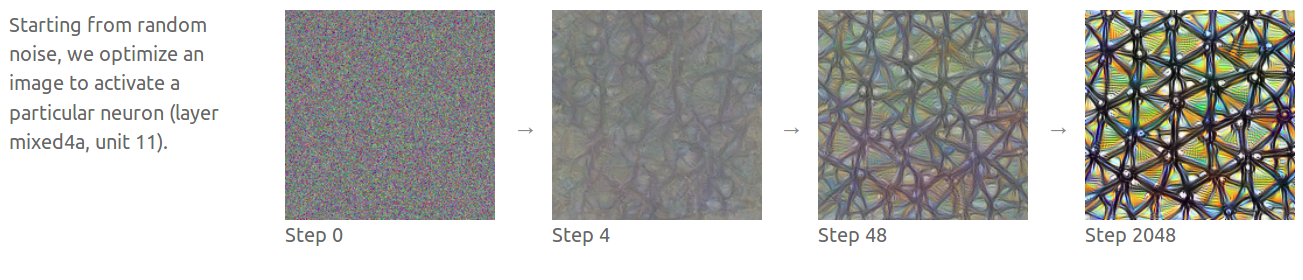
\includegraphics[width=0.8\linewidth]{randopt}
	\caption{\textit{Activation maximization method.} The process starts with random noise and performs gradient ascent to find the input sample that maximizes the activation of a unit (or a channel, in this case). Figure reproduced from \cite{Olah2017}.}
	\label{fig:randopt}
\end{figure}

This technique brings the benefit of keeping the most relevant bits that are captured by the unit and discard all non-relevant information. It can also be easily applied to groups of neurons, such as channels, layers or other arbitrary collections, and it can be applied at different stages of the training process in order to visualise how the learning evolves. However, it also has some drawbacks: the optimization function is non-convex, and the algorithm can arrive at different local minima, so special techniques need to be added to find all the relevant ones (\cite{Nguyen2016,Olah2017}); the gradient ascent requires setting a stopping criterion and a learning rate, and the process can produce highly unrealistic samples. This last issue could be potentially mitigated by the introduction of duly prior constraints, such as ``neighboring pixels needing to be correlated" in natural images (\cite{Mordvintsev2015}). \cite{Montavon2018} materialise the inclusion of this prior knowledge in an \textit{expert term} in Equation \ref{eq:opt} and argue that its determination is crucial in the resulting sample, and suggest seeking slightly under-fitting expert terms.    
\begin{figure}
	\centering
	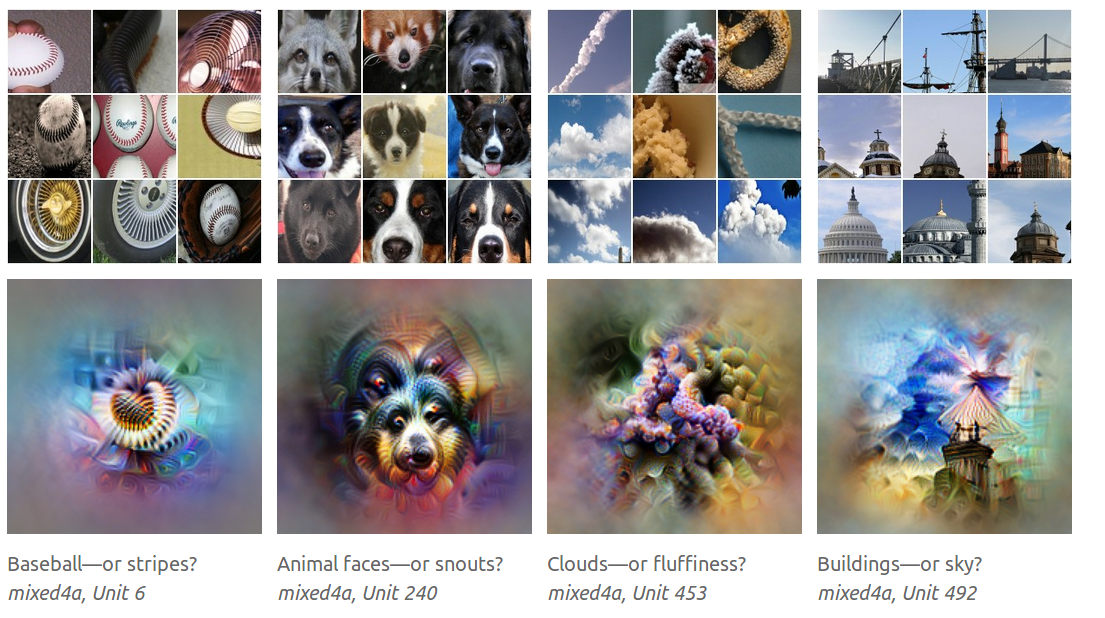
\includegraphics[width=0.7\linewidth]{optimization}
	\caption{\textit{Maximally activating samples from training/test set (above) and activation maximization outcome (below) for four different units.} A single activation maximization local minimum does not capture all the variety of the neuron, so a multi-faceted set of them should be sought. Figure reproduced from \cite{Olah2017}.}
	\label{optimization}
\end{figure}


\subsection{Saliency maps (or how to assign importance scores)}

Saliency maps are a series of techniques that are developed in order to reveal which parts of an input sample are mainly responsible for the output decision that the network makes. They can be a powerful tool both for spotting spurious rules learned by the system (in cases where we can easily judge whether a result is wrong) and learning more about the underlying processes (when we cannot explain the reason of a result, as it is common in biology). An example of a saliency map visualisation can be seen in Figure \ref{fig:deeptaylor}.

\begin{figure}
	\centering
	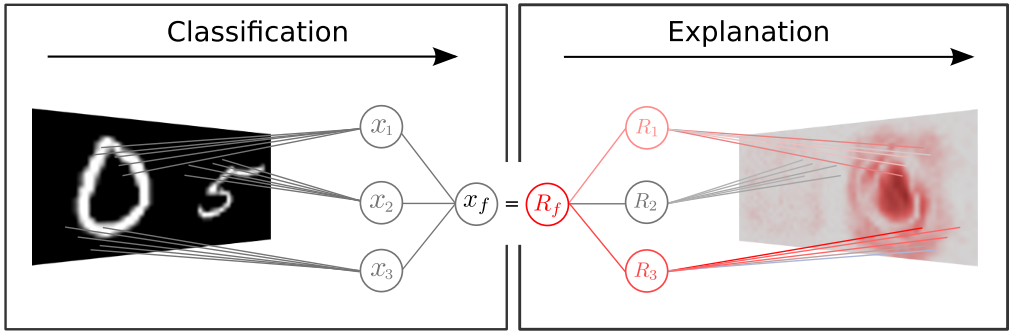
\includegraphics[width=0.7\linewidth]{Figures/deeptaylor}
	\caption{\textit{Basic sample of a saliency map.} Here, the network is detecting the digit zero (on the left) and the pixels that contributed to the classification are highlighted (on the right). Image reproduced form \cite{Montavon2017}.}
	\label{fig:deeptaylor}
\end{figure}


The most straightforward approach to achieve this goal is performing a sensitivity analysis, i.e. making modifications of the input sample and register how variations in each input (or combinations of them) affect the output of the system. These techniques can be applied to other units different from the post-softmax to give ideas of intermediate layers as well. They can be grouped by the name \textit{perturbation-based approaches}, and they all face the same problem: when the input space is moderately big, exploring a decent amount of variations and combinations is intractable, or conspicuously computationally expensive at the least. A second concern relates to its inability to capture the importance of neurons that are already saturated. One example of such methods specifically applied to CNNs is DeConvNets (\cite{Zeiler2014}), a machine that assigns scores to specific patches of the input image based on their contribution.

The second series of approaches that mostly overcome the computational problems are based in back-propagation. The most intuitive idea behind them is that the gradient of an input already tells you its sensitivity (how much the output will change from a small change in the input), and it can be calculated on a single back-prop operation instead of performing a profligate number of feed-forward passings with small variations in the inputs (\cite{Shrikumar2017}). It can be thought as a linear approximation of the function around the sample point $x_0$ by applying first-order Taylor expansion, as introduced by \cite{Simonyan2014}:
\begin{align}
f(x) \approx w x + b \; , \nonumber \\
w = \left. \frac{\partial f}{\partial x} \right|_{x_0} \; .
\end{align}

Some other similar methods were developed, with their main differences residing in the treatment of ReLUs in the back-propagation process, such as \textit{guided backpropagation} (\cite{Springenberg2014}). However, they do not give solid explanations for assigning importance since they do not hold basic principles such as conservation (all the importance scores at any layer should sum up to the output score). This principle was later introduced by \cite{Bach2015} with the \textit{Layer-wise Relevance Propagation} (LRP) method, although it has been later discussed that the rules it follows are mainly heuristic and more principled ways of choosing the rules have been suggested (\cite{Montavon2017}). It was later proven that these rules were equivalent to having the element-wise multiplication of the original saliency maps by the input itself (\cite{Shrikumar2016}). Finally, a last wave of methods proposes including a reference point and hence properly accomplishing the Taylor approximation. Main examples are \textit{integrated gradients} (\cite{Sundararajan2017}), Deep Taylor Decomposition (\cite{Montavon2017}), and DeepLIFT (\cite{Shrikumar2017}). They overcome problems of previous methods such as saturation or discontinuities in the gradients.

\section{Deep Learning in biology}

Recent advances in measuring techniques have produced vast amounts of biological data, which usually is highly dimensional and reflects incredibly complex underlying processes. Such settings demand more powerful models than before, and deep learning has found there a natural field in which to be applied. Among the most prominent application domains in which it has been successfully implemented are images (bioimaging, medical imaging), brain/body-machine interfaces (\textit{BMI}s) and \textit{omics} (\cite{Mahmud2018}). The omics term includes research of sequence data at the cellular level, namely the DNA (\textit{genomics}), RNA (\textit{transcriptomics}), proteins (\textit{proteomics}), and their interaction (\textit{multiomics}). Sequential data is particularly interesting for deep learning since it is one kind of problems in which it excels, particularly with the application of RNNs and CNNs. They have been widely employed for structural annotation of the DNA chain (\cite{Jones2017}), protein classification (\cite{Min2017}), splicing code (\cite{Mamoshina2016}) and transcription factors (\cite{Ching2017}), among others.

\subsection{CNNs on biological sequence data}
As it has been mentioned in Section \ref{sect:cnn}, CNNs are mostly useful on data which is spatially correlated, which is the case of sequential data. Some reasons for this is that they can accept input sequences of arbitrary size and they can capture motifs in them irrespectively of where they are located (\cite{Jurtz2017}). While applying convolutions to 2D input images is a well-known task, it is not as common to apply to one-dimensional data. It is nevertheless fairly intuitive. Filters cover the whole depth (channels) of the data and have variable width depending on the number of neighbouring positions that we want them to capture. Filters slide only in the direction of the sequence, with possibilities of different strides and padding, as in normal 2D convolution. A 1D convolution operation transforms the 2D input sequence $x$ with length $L$ and depth $D$ into the 1D feature sequence~$z$. Each element of $z$ is computed as
\begin{equation}
z_i = f\left( \sum_{k=0}^{D} \sum_{j=-h}^{h} w_{jk} \cdot x_{i+j,k} + b \right) \; ,
\end{equation}
with $h$ being the half-width of the filter, $D$ the total depth of the input, $w_j$ and $b$ the weight and bias variables of the filter and $f$ the non-linear activation function. Many simultaneous convolutions operations can be performed at any layer with varying parameters in order to obtain a 2D set of feature maps that will serve as input for the next layer.

While signals as inputs contain real-value data, categorical sequences ---such as DNA, amino-acid chains, or characters in a text classification task (\cite{Zhang2015})--- are presented in their one-hot version, defining the depth of protein chains as 21 (different possible amino-acids) and four for DNA and RNA (the four bases). Some extra depth can be added with additional known features of the element, such as solvent accessibility or \textit{pssm} values in the case of amino-acids.

There are two main ways in which to apply convolutions to sequence data depending on the problem: structural annotation or sequence classification. The first kind of problems requires the network to assign a specific label or value to each of the positions in the input sequence, and therefore the network has to maintain the input length throughout the convolution layers, which can be done with half padding and strides of one. The second problem produces a single output (classification) for a whole sequence. Doing so requires a shrinking process that cannot be achieved by standard means of convolution and pooling operations since they have fixed reduction sizes and input sequences may have varying lengths. The final step reduction can be achieved by a global max-pooling that retrieves the highest value of the sequence feature map at a single channel, therefore producing a fixed-size vector that can be fed to a soft-max layer (\cite{Jurtz2017}).

%\begin{figure}[h]
%    \centering
%    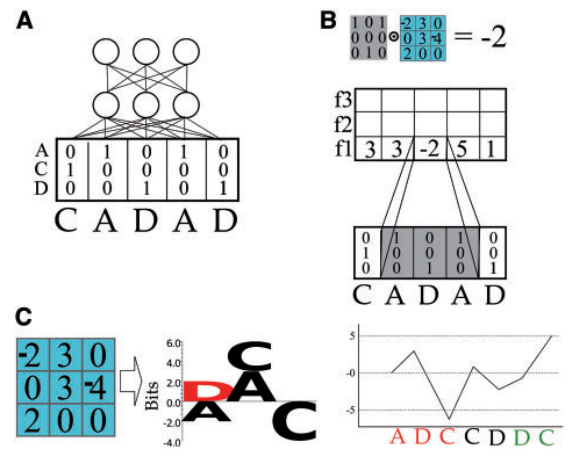
\includegraphics[width=0.7\linewidth]{cnnbio}
%\end{figure}

\subsection{Interpretability techniques on biological sequence problems}
The biomedical field is one with special pressures into having interpretable systems. On the one hand, the costs of false predictions is expensive when it comes to diagnosis, and finding spurious rule is of particular importance. On the other hand, inspecting what networks are learning can provide with valuable information about the underlying biological processes. Unlike with image classification processes, sequence properties relies sheerly on the arrange of the limited number of possible elements, and being able to find which motifs lead to certain outputs is of particular relevance. Apart from this, having non-interpretable models can impinge the trust of experts in the biomedical field and deter them for using the more advanced deep learning versions since they are not able to understand them.

\subsubsection*{Feature visualisation methods}
As discussed in Section \ref{sect:featvis}, a first approximation to visualise hidden features is to inspect the filters of the first layer of a CNN. It gives a first idea of which ground features the network is building but is unable to go further than that, so it remains relevant only for shallow structures. When it comes to sequential biological data, an efficient way to convey the information that is also familiar for biology experts are the \textit{Seq2Logo} charts (\cite{Thomsen2012}). 1D~convolutional filters can be represented in this way by pairing up their values with the amino-acid of the one-hot row they cover. Two samples of such representations can be seen in Figure \ref{fig:seqlogo}.

\begin{figure}
	\centering
	%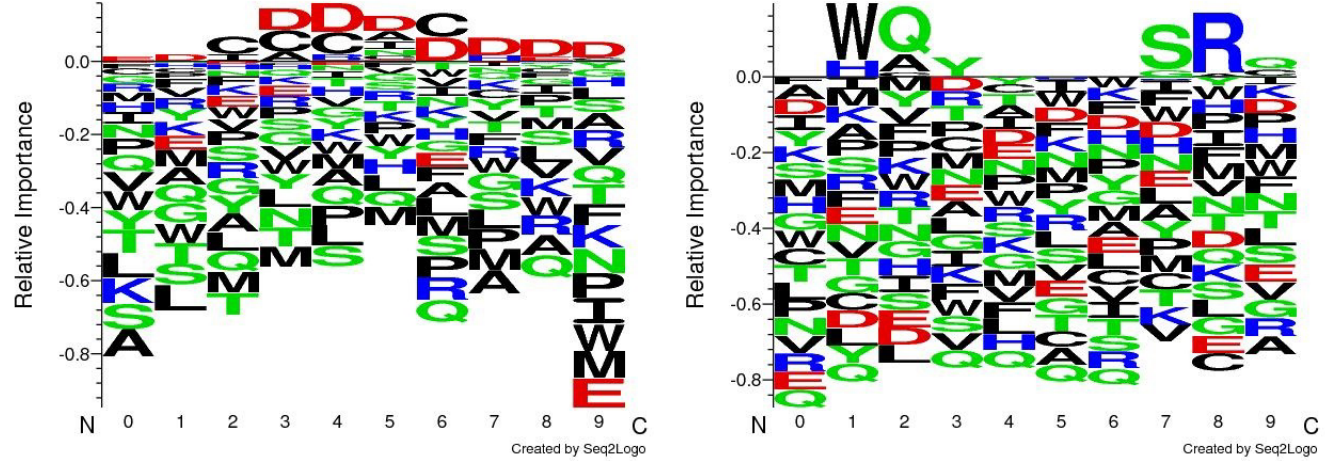
\includegraphics[width=0.7\linewidth]{Figures/seqlogo}
	\subfigure{
		\includegraphics[width=0.4\linewidth]{Figures/FirstFilter}
		\label{Figure:figsubex:left}
	}
	\subfigure{
		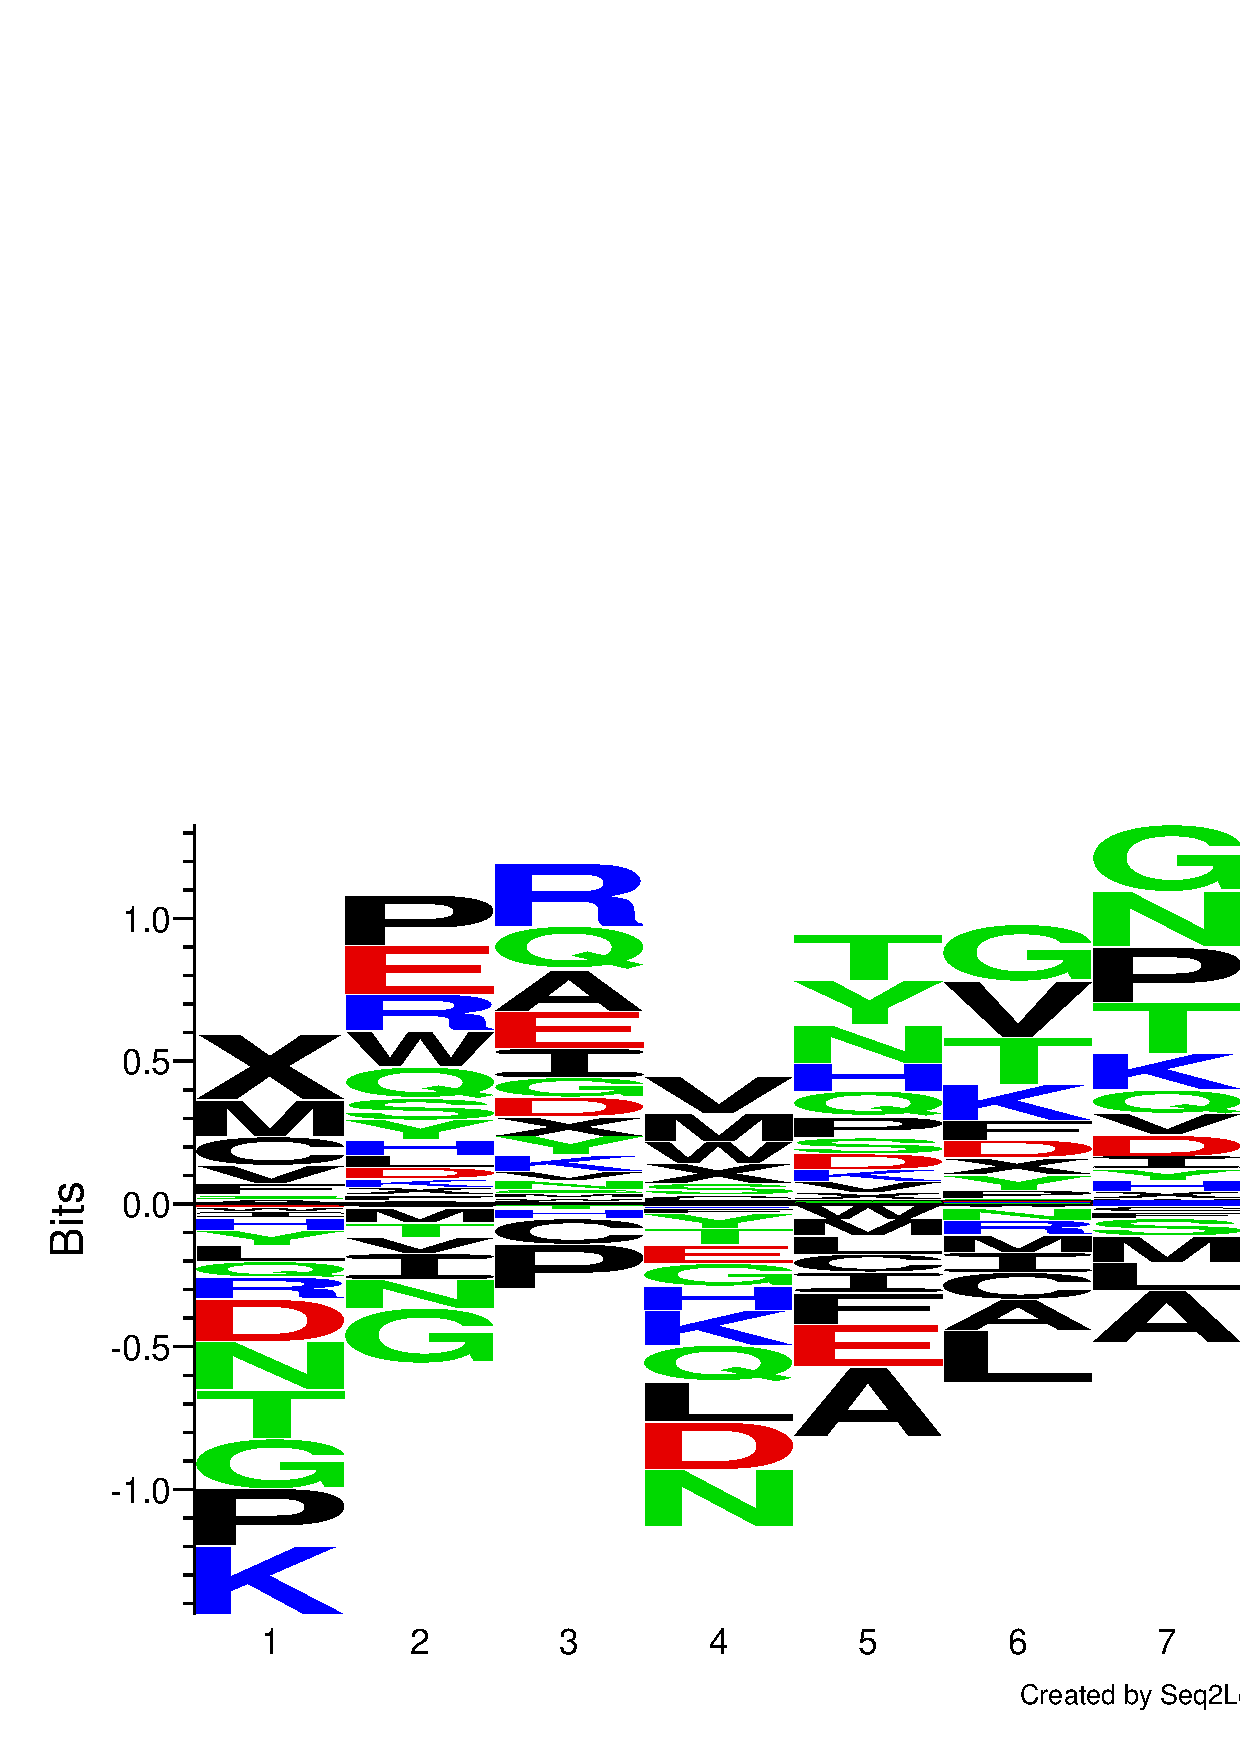
\includegraphics[width=0.4\linewidth]{Figures/FirstFilter2}
		\label{Figure:figsubex:right}
	}
	\caption{\textit{Two first-layer filters for a protein sequence problem shown as Seq2Logo.} The $x$ axis represents the span of the filters, which is seven in both filters presented here. While the left filter captures the appearance of specific amino-acids at the sides and not the centre, the right one resembles more an edge detector, with many amino-acids with different signs at each side.}
	\label{fig:seqlogo}
\end{figure}

Some works have gone further by applying activation maximisation techniques as well. \cite{Fontal2017} attempted to apply it for protein subcellular localisation prediction by applying gradient ascent on the pre-softmax units ($s_i$) with an L2 regularisation parameter, $\lambda$:
\begin{equation}
\arg\max \: s_i(x) + \lambda \left\| x \right\|_2^2 \; .
\end{equation}
\cite{Lanchantin2016} applied it to TF binding-site classification of genetic sequences with the same method (applied to post-softmax) and found that 30\% of them could be found in public motif databases. As another means of visualising hidden layer features, \cite{Lanchantin2016} also included temporal output scores for the RNNs models.

\subsubsection*{Saliency maps}
As a simplified version of saliency maps, \cite{Alipanahi2015} and \cite{Quang2016} spotted the segment in the input genetic sequence that had the highest activation of the first-layer filters and compared them to known motifs. This approach only makes sense as long as the network has a single layer, but cannot be applied to deeper networks.

\cite{Alipanahi2015} and \cite{Zhou2015} showed how genetic mutations affected the output, which is a natural way of performing perturbation-based approaches for the field. \cite{Umarov2017,Fontal2017} substituted small windows of the sequence ---by random genetic code and the general amino-acid X, respectively--- and assessed the differences in the output along the sequence by sliding these windows. \cite{Kelley2016} introduced in the centre of DNA sequences known motifs. All of these can be categorised in the \textit{perturbation-based approach} group, therefore need high computational times and cannot be exhaustive enough: how many window sizes and up to which range should be tried to localise the influence accurately?.

Gradient-based approaches have barely been translated to the biological field yet. \cite{Lanchantin2016} include saliency maps with the form of gradient * input for TF binding sites classification, extracted the size nine window with the highest score from each saliency map and compared them with a database of known motifs, matching almost half of the motifs thus produced. Figure \ref{fig:demo} shows a sample of their saliency maps along with other interpretability methods.

\begin{figure}
	\centering
	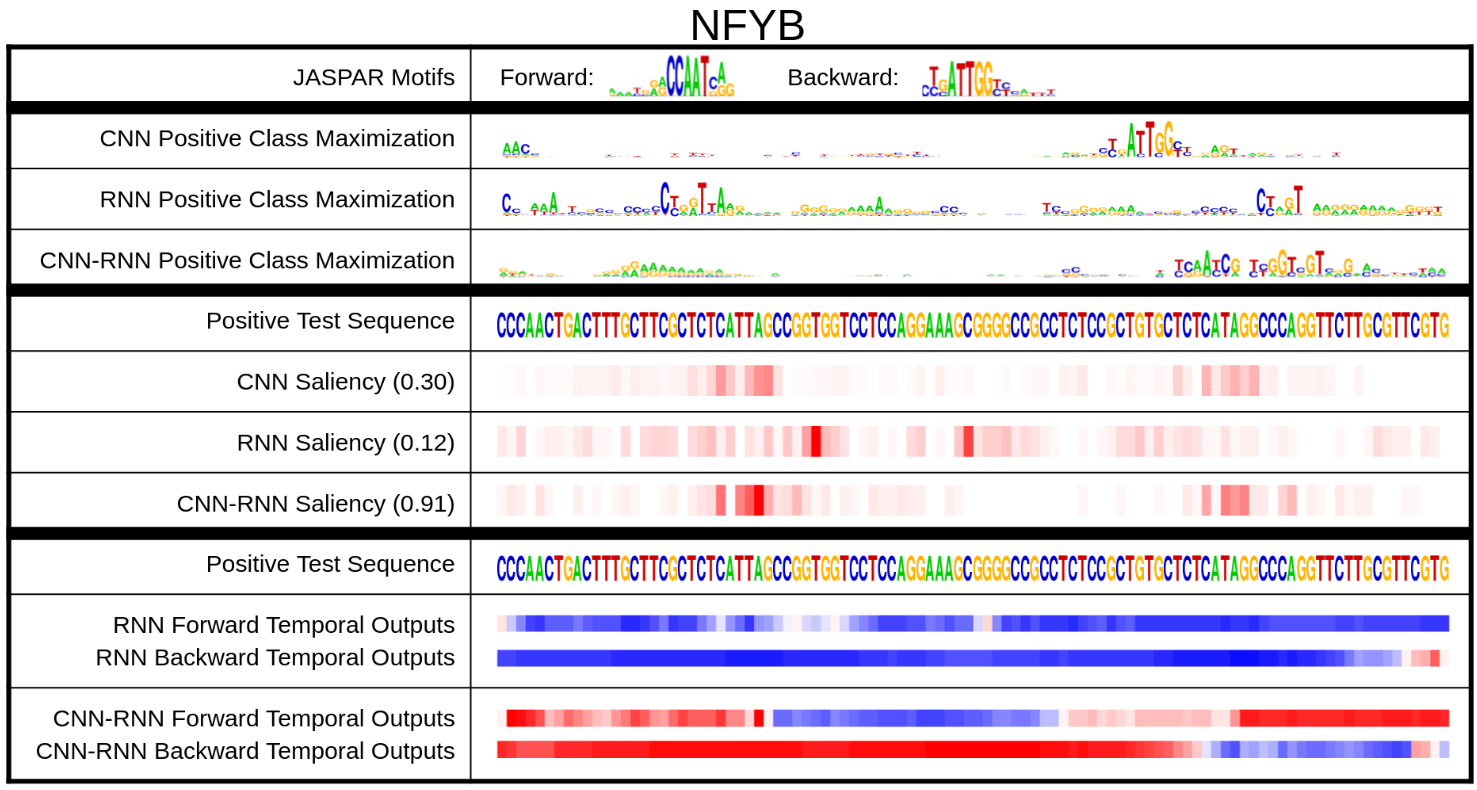
\includegraphics[width=0.8\linewidth]{Figures/demo}
	\caption{\textit{Deep Motif dashboard including varied interpretability techniques for TF Binding Site classification.} This figure includes activation maximization methods (top), saliency maps (middle) and temporal outputs (bottom) for CNNs, RNNs, and a combination of both. Figure reproduced from \cite{Lanchantin2016}.}
	\label{fig:demo}
\end{figure}

\cite{Shrikumar2017} developed the new back-propagation based technique \textit{DeepLIFT} and simulated a motif detection task within a genomic sequence to prove their effectiveness. \cite{Finnegan2017} utilised Markov chain Monte Carlo methods to withdraw samples from the maximum entropy distribution and assessed importance score by looking at the variance of the samples at each position. This technique was applied for previously trained DNA-protein binding CNN and proved to be better than DeepLIFT.

All these methods address classification problems where there is a single output (classification task) for the whole sequence, but, to the best of my knowledge, interpretability techniques have not been applied to structural tagging problems.


\section{Protein Secondary Structure Prediction}

%TODO: Read through \cite{Wang2016}'s bibliography 1-12 and improve this section + add references.

Secondary structure prediction is a long-time studied problem that spans more than 50 years already (\cite{Pauling1951}). It has gone through many different stages as mathematical and computational methods evolved, being recently benefited from deep learning as well, to the point of approaching the theoretical accuracy limit (\cite{Heffernan2017})\footnote{Since there is 12\% structure homology between proteins (\cite{Rost2001}).}. Due to its long history, it has also been suggested that it effectively works as a problem benchmark for new techniques dealing with sequence data.

Predicting the secondary structure of a protein purely from its sequence can be seen as a middle step for tackling the much harder problem of predicting 3D structure. This last problem is of great importance in the biomedical field since protein structures are the principal indicator of their function, and obtaining this information can be of great use at drug design, disease treatment or early diagnosis, among others. However, due to the molecular scale, these structures cannot be easily measured, and any attempt to do so remains costly. A more feasible alternative is utilising computational tools to predict protein structures from amino-acid sequences alone, as these can be easily obtained from DNA sequencing and they are widely available on heavily annotated public databases (\cite{Dill2012}). From the nearly 85 million proteins whose sequences are known (\cite{Hattori2017}), we only know the structure of about 130 thousand (\cite{Magnan2014}).

\subsection{Input features}
The input to the system is an amino acid chain of length $l$. Since amino acids can be of any of 21 categories\footnote{There are 20 standard types while amino-acid X is commonly used for representing all the unknown or non-standard ones (\cite{Zhou2018}). Other ways of handling non-standard amino-acids are also possible (\cite{Fang2017}).}, the most natural way is to treat them as one-hot vectors, forming an input matrix of 21x$l$. Other features of the amino-acids ---such as solving accessibility or other physio-chemical properties (\cite{Fauchere1988})--- could also be added to the end of the vector, adding thus extra-information that could be potentially important for making the classification. A typical approach involves inspecting the sequence by taking \textit{n-grams} (i.e. fragments of size $n$) and classify the middle amino-acid with classical machine learning algorithms such as support vector machines (\textit{SVM}s). This approach was also held by the first neural networks applied to the problem. With the arrival of CNNs and RNNs, the whole input matrix is fed to the system, as they allow for inputs of varying lengths.

A key turning point for prediction performance appeared when Position Specific Substitution Matrices (\textit{PSSM}) were added as extra features (\cite{Yang2018}). These values are originated from sequence alignment with \textit{PSI-BLAST} (\cite{Altschul1997}) and express the probability of finding sequences that have a specific amino-acid substituted by another. Each amino-acid of the sequence has then 21 extra features that represent how likely are each of the 21 types of amino-acids found on similar sequences, which gives valuable information about mutations that do not change the structure of the protein (and hence its function) and are then kept by evolution. In order to make most of this information with machine learning algorithms, it is usually filtered through a sigmoid function that the values between 0 and 1 (\cite{Jones1999}), although it can be further normalised to zero mean and one standard deviation (\cite{Busia2017}).

The combination of one-hot encoded (sparse) along with \textit{pssm} (dense) features brings some problems for conventional machine learning algorithms: the dense part carries more information than the sparse one, so the weights associated to this part of the input vector learn much faster. \cite{Li2016} and \cite{Zhou2018} had the one-hot side of the input embedded into a denser representation through an MLP ---as it is common in natural language processing (\cite{Mesnil2015})---, but reported only a small marginal performance improvement in doing that (0.5\% and 0.4\% Q8 accuracy, respectively). \cite{Spencer2015} reported an improvement of 2\% Q3 accuracy by directly not including the one-hot amino-acids in their model, relying purely on the \textit{pssm} scores.

\subsection{Targets}
Broadly, there are three kinds of local structures based on the hydrogen bonds formed between the amino-acids: $\alpha$\textit{-helix}, $\beta$\textit{-sheet}, and \textit{coil}, which includes everything else. These were proposed by \cite{Pauling1951} when the protein secondary-structure problem was first defined and have been the targets mostly used in the secondary structure prediction problem, and it is generally referred to as \textit{Q3}.

A finer classification schema developed by \cite{Kabsch1983}, the \textit{Dictionary of Secondary Structure of Proteins (DSSP)}, focuses in two smaller sub-units: \textit{turns} and \textit{bridges}. Repeating turns would form helices, and consecutive bridges create \textit{ladders}, which in turn form sheets. Depending on how many of them are found together, different kinds of helices or strands could form, leading to a finer classification that comprehends eight classes in total: three kinds of helices, two sheets, and three coils. Having a more precise classification increases the complexity of the problem and has therefore been the focus of recent, more powerful deep learning approaches. This classification schema is commonly referred to as \textit{Q8}, and an algorithm for its classification was also developed by \cite{Kabsch1983}. A detailed list of the classes can be seen in Table \ref{tab:q8}.

%"The secondary structures (SS) of a protein represent the local conformations of a three-dimensional structure. There are three main secondary structures: α-helices [8], β-sheets [9] and turns [10]." \cite{Hattori2017}

\begin{table}[h]
	\begin{tabular}{cc|cc|c}
		\multicolumn{2}{c}{\textbf{Q3 grouping}} & \multicolumn{2}{c}{\textbf{Q8 grouping}} &  \textbf{Explanation} \\ 
		&   & $\alpha$-helix & H & Helix with 4 turns \\ 
		$\alpha$-helix    & H & $3_{10}$-helix & G & Smaller helix with 3 turns \\ 
		&   & $pi$-helix      & I & Bigger helix with 5 turns. Not as common.\\ \hline
		\multirow{2}{*}{$\beta$-sheet}    & \multirow{2}{*}{B} & $\beta$-bridge & B & Isolated $\beta$-bridge \\ 
		&                       & $\beta$-strand & E & Participates in $\beta$-ladders \\ \hline
		&   & Turn & T & Turns that do not reach the minimum to be a helix \\ 
		Coil    & C & Bend & S & Curved piece \\ 
		&   & Loop & L & Sometimes also categorized simply as coil (C)
	\end{tabular}
	\label{tab:q8}
	\caption{\textit{Targets for the secondary structure prediction problem.} The simpler way of 3-class grouping was further expanded into eight classes by \cite{Kabsch1983} in their Dictionary of Secondary Structure or Proteins (DSSP).}
\end{table}

The natural way to format them for prediction is their transformation in one-hot vector form, with a softmax function as the last layer of the network as a means to provide with posterior probabilities, p($Q|x$). Networks are typically trained using cross-entropy between targets and predictions, and the most commonly used performance score is accuracy, as the percentage of residues correctly classified. Some other performance measures include per-class precision and recall (\cite{Wang2016}), ROC Area Under the Curve (\cite{Hattori2017}), Matthews correlation coefficient (\cite{Fang2017}), Person's Correlation Coefficient (\cite{Jurtz2017}), or Segment of Overlap (\cite{Wang2016}).

\subsection{State of the art}
Secondary structure prediction problem has a long history, with first approaches mainly rooted in statistics (\cite{Chou1974}). Breakthroughs can be found with the first implementations of neural networks (\cite{Qian1988}) and the inclusion of \textit{pssm} values as inputs (\cite{Rost1993}). Early neural network approaches included mainly shallow networks with a single hidden layer (\cite{Qian1988,doi:10.1016/0014-5793(88)81066-4,Rost1993}) and two such networks stacked at most (\cite{Jones1999,Dor2007}). A new generation of deep learning started recently with \cite{Zhou2014} building Generative Stochastic Network with two hidden layers and later works that already included five or more, with some even reaching more than 30 (\cite{8371925,Fang2017}). These deeper models introduced new major improvements while being more flexible in merging information from local and more distant contexts. Earlier approaches typically used the n-grams or sliding window approach. CNNs, although with a similar principle, have a rather pyramidal structure, being able to increase the span of their action (see Figure \ref{fig:cnnwang}). RNNs can capture even longer interactions and are deep in the sense of having the information at one timestep repeatedly re-processed in many later time steps. Table \ref{tab:HoF} collects the best results achieved for Q8 in the last few years. All results are measured on the CB513 benchmark dataset first introduced by \cite{Zhou2014}. All state-of-the-art algorithms are based on deep learning networks, either in the form of CNNs, RNNs, or both combined.

\begin{figure}
	\centering
	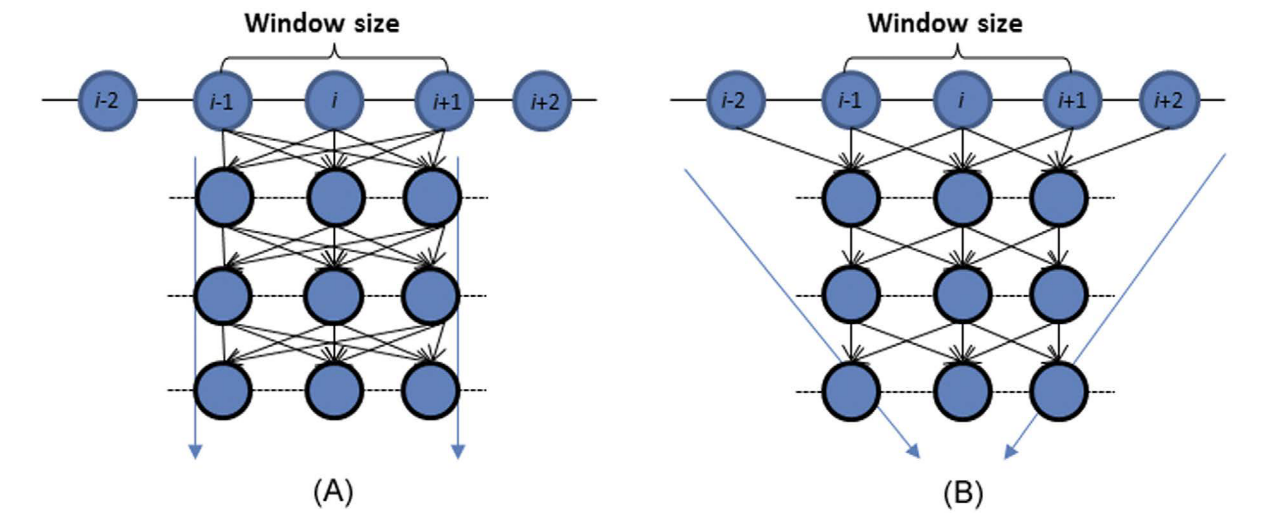
\includegraphics[width=0.8\linewidth]{cnnwang}
	\caption{\textit{Improvements of CNNs over fixed-window sliding.} While for MLP are not as flexible when at capturing information from different contexts (left), CNNs are able to merge local information at the lower layers with longer-range info at upper layers (\cite{Busia2017}). Furthermore, increasing the depth expands the window size without adding much complexity to the model. Figure reproduced from \cite{Wang2016}.}
	\label{fig:cnnwang}
\end{figure}

\begin{table}
	\begin{tabular}{cccc}
		\textbf{Names} & \textbf{Q8} & \textbf{Architecture} & \textbf{Date} \\
		\cite{Zhou2014}    & 66.4\%     & \textbf{CGSN}             & 2014 \\ 
		\cite{Magnan2014} & 66.5\% & SSPro (BRNN) & 2014 \\
		\cite{Sønderby2014}    & 67.45\%     & LSTM             & 2014     \\ 
		\cite{Wang2016} & 68.3\% & \textbf{DeepCNF}     & Jan 2016 \\ 
		\cite{Li2016}    & 69.7\%     & \textbf{DCRNN}         & Apr 2016 \\
		\cite{Lin2016}     & 68.4\%     & \textbf{MUST-CNN}         & May 2016 \\
		\cite{Busia2017}& \textbf{71.4\%}& \textbf{Deep3I+conditioning}& Feb 2017 \\
		\cite{Hattori2017} & 68.0\%    & DBLSTM        & May 2017 \\
		\cite{Jurtz2017} & 70.2\%    & \textbf{LSTM+CNN}         & Aug 2017 \\
		\cite{Johansen2017} & 70.9\% & BGRU-CRF & Aug 2017 \\
		\cite{8371925} & \textbf{71.1\%} & \textbf{DeepNRN+Deep3I} & Nov 2017 \\
		\cite{Zhou2018} & 70.3\% & \textbf{CNN+highway} & Jan 2018 \\
		\cite{Fang2017}& 70.63\% & \textbf{MUFold-SS (Deep3I)}&Feb 2018\\
	\end{tabular}
	\label{tab:HoF}
	\caption{\textit{State-of-the-art Q8 results on benchmark CB513.} All networks include some sort of deep learning architecture. Architectures in bold indicate some sort of CNN were included. Best Q8 results are marked in bold.}
\end{table}